% XeLaTeX

\documentclass{article}
\usepackage{ctex}
\usepackage{xypic}
\usepackage{amsfonts,amssymb}
\usepackage{multirow}
\usepackage{geometry}
\usepackage{graphicx}
\usepackage{listings}
\usepackage{lipsum}
\usepackage{courier}
\usepackage{fancyvrb}
\usepackage{etoolbox}


\linespread{1.2}
\geometry{left=3cm,right=2.5cm,top=2.5cm,bottom=2.5cm}

\makeatletter
\patchcmd{\FV@SetupFont}
  {\FV@BaseLineStretch}
  {\fontencoding{T1}\FV@BaseLineStretch}
  {}{}
\makeatother

\lstset{basicstyle=\small\fontencoding{T1}\ttfamily,breaklines=true}
\lstset{numbers=left,frame=shadowbox,tabsize=4}
%\lstset{extendedchars=false}
\begin{document}

\title{实验三 \text{ } 组合逻辑电路分析与设计 \text{ } 实验报告}
\author {16337233 王凯祺}
\maketitle

\section{实验目的}

1. 掌握组合逻辑电路的分析方法,并验证其逻辑功能

2. 掌握组合逻辑电路的设计方法,并能用最少的逻辑门实现之

3. 熟悉示波器和逻辑分析仪的使用

\section{实验原理}

组合逻辑电路的设计:按照具体逻辑命题设计出最简单的组合电路。

1. 根据给定事件的因果关系列出真值表

2. 由真值表写函数式

3. 对函数式进行化简

4. 画出逻辑图,并测试逻辑功能

\section{实验仪器}

数字电路实验箱、逻辑分析仪、74LS00、74LS86、74LS197

\section{实验内容}

设计一个代码转换电路,输入为 4 位 8421 码,输出为 4 位格雷码。

\newpage

\section{实验设计}

\subsection{真值表}

\begin{table}[!hbp]
\begin{tabular}{|c|c|c|c||c|c|c|c|}
\hline
A3 & A2 & A1 & A0 & Y3 & Y2 & Y1 & Y0 \\
\hline
\hline
0 & 0 & 0 & 0 & 0 & 0 & 0 & 0 \\
\hline
0 & 0 & 0 & 1 & 0 & 0 & 0 & 1 \\
\hline
0 & 0 & 1 & 0 & 0 & 0 & 1 & 1 \\
\hline
0 & 0 & 1 & 1 & 0 & 0 & 1 & 0 \\
\hline
0 & 1 & 0 & 0 & 0 & 1 & 1 & 0 \\
\hline
0 & 1 & 0 & 1 & 0 & 1 & 1 & 1 \\
\hline
0 & 1 & 1 & 0 & 0 & 1 & 0 & 1 \\
\hline
0 & 1 & 1 & 1 & 0 & 1 & 0 & 0 \\
\hline
1 & 0 & 0 & 0 & 1 & 1 & 0 & 0 \\
\hline
1 & 0 & 0 & 1 & 1 & 1 & 0 & 1 \\
\hline
1 & 0 & 1 & 0 & 1 & 1 & 1 & 1 \\
\hline
1 & 0 & 1 & 1 & 1 & 1 & 1 & 0 \\
\hline
1 & 1 & 0 & 0 & 1 & 0 & 1 & 0 \\
\hline
1 & 1 & 0 & 1 & 1 & 0 & 1 & 1 \\
\hline
1 & 1 & 1 & 0 & 1 & 0 & 0 & 1 \\
\hline
1 & 1 & 1 & 1 & 1 & 0 & 0 & 0 \\
\hline

\end{tabular}
\end{table}

\subsection{卡诺图}

\subsubsection{Y3}

\begin{figure}[!hbp]
  \centering
  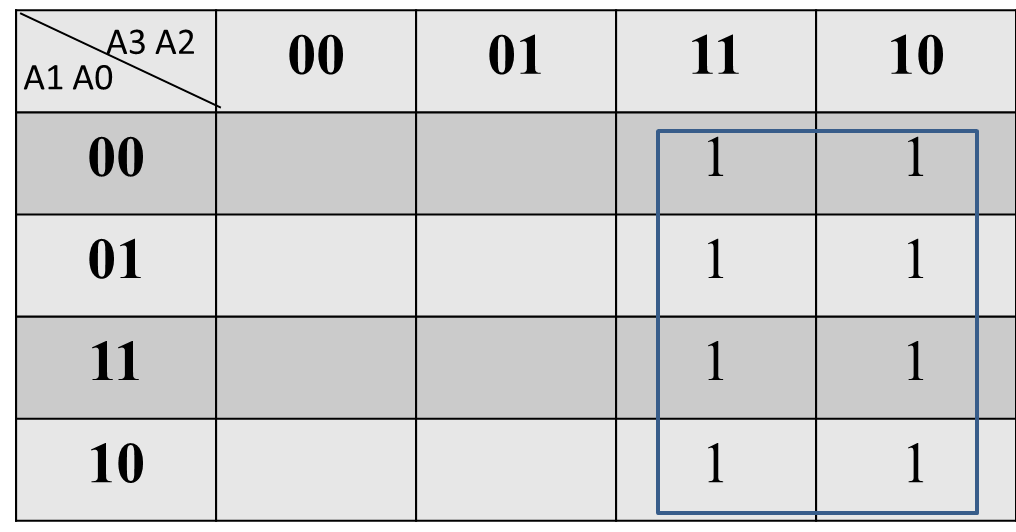
\includegraphics[scale=0.45]{S4.png}
\end{figure}

$Y3 = A3$

\newpage

\subsubsection{Y2}

\begin{figure}[!hbp]
  \centering
  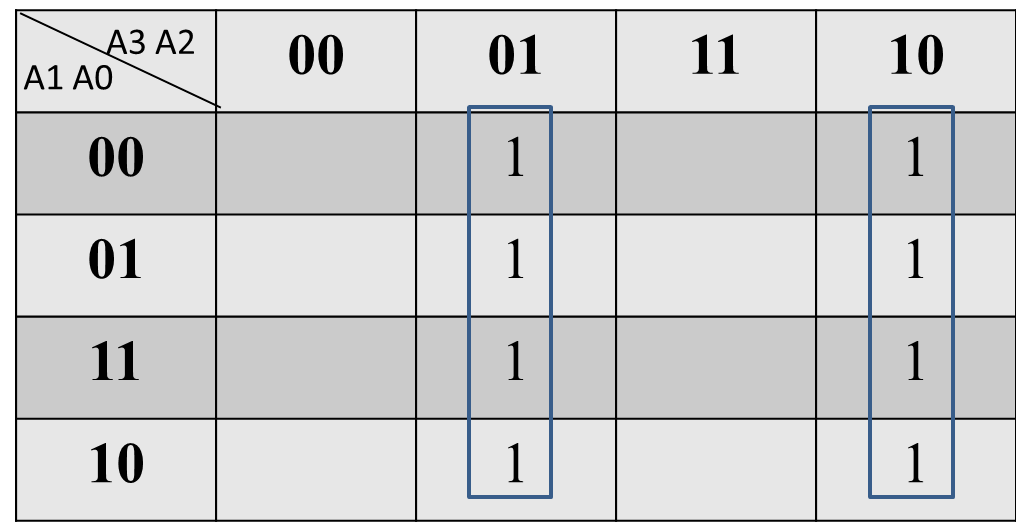
\includegraphics[scale=0.45]{S5.png}
\end{figure}

$Y2 = A3 * \overline{A2} + \overline{A3} * A2 = A3 \oplus A2$

\subsubsection{Y1}

\begin{figure}[!hbp]
  \centering
  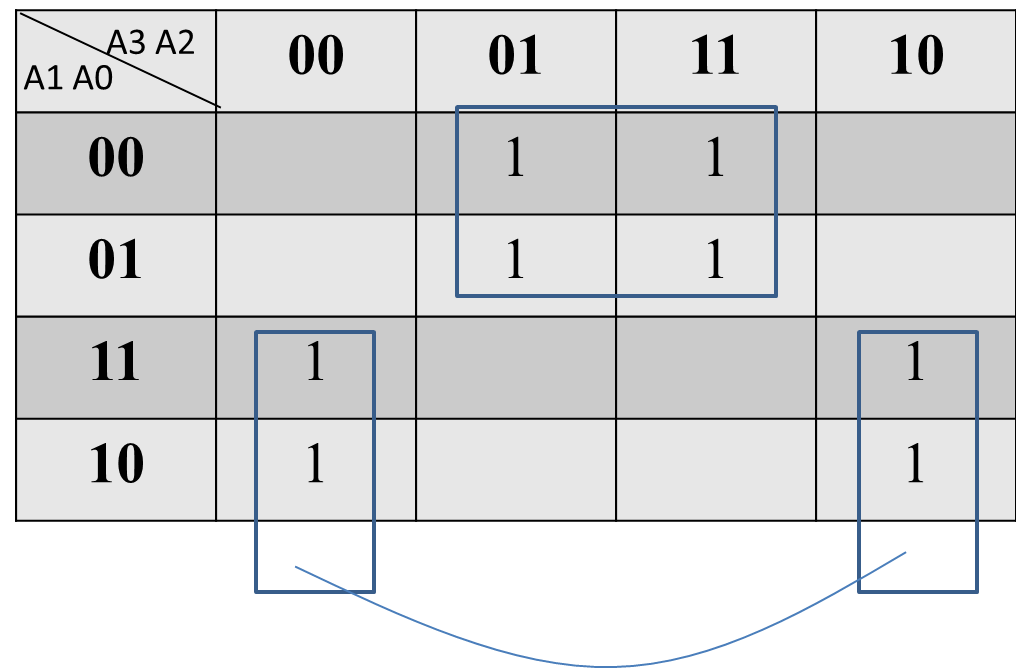
\includegraphics[scale=0.45]{S6.png}
\end{figure}

$Y1 = A2 * \overline{A1} + \overline{A2} * A1 = A2 \oplus A1$

\subsubsection{Y0}

\begin{figure}[!hbp]
  \centering
  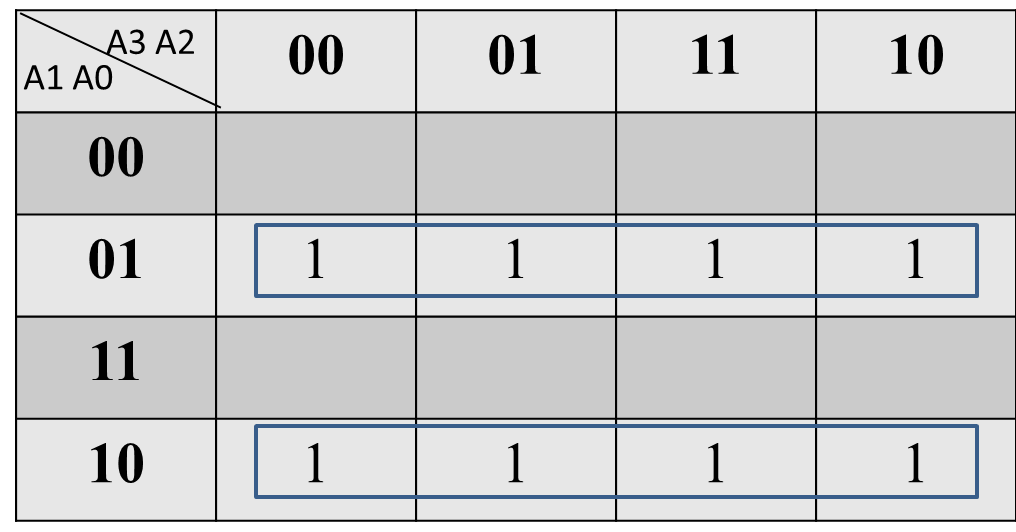
\includegraphics[scale=0.45]{S7.png}
\end{figure}

$Y0 = A1 * \overline{A0} + \overline{A1} * A0 = A1 \oplus A0$

\subsection{表达式}

$Y3 = A3$

$Y2 = A3 \oplus A2$

$Y1 = A2 \oplus A1$

$Y0 = A1 \oplus A0$


\section{Proteus 电路设计}

\begin{figure}[!hbp]
  \centering
  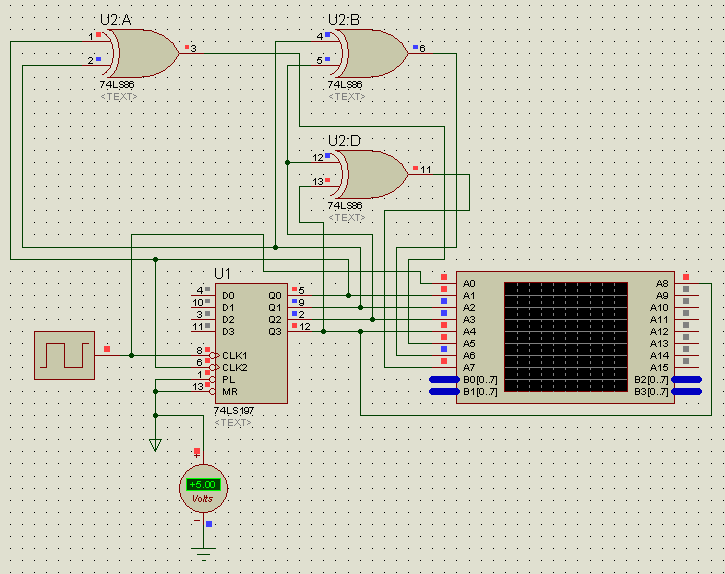
\includegraphics[scale=0.45]{S1.png}
\end{figure}

\begin{figure}[!hbp]
  \centering
  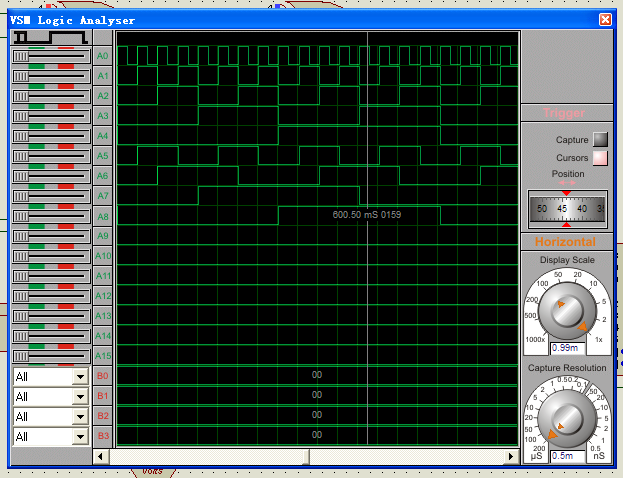
\includegraphics[scale=0.45]{S2.png}
\end{figure}

上图中, $A_0$ 表示时钟信号, $A_1$ 表示输入最低位, $A_4$ 表示输入最高位, $A_5$ 表示输出最低位, $A_8$ 表示输出最高位。

\newpage

\section{静态测试}

用逻辑开关模拟二进制代码输入,并把输出接 0-1 显示器,检查电路是否正常工作。

\section{动态测试}

将十六进制计数器 74LS197 的输出连接到代码转换的输入端,作为 8421 码的输入。

\begin{figure}[!hbp]
  \centering
  \includegraphics[scale=0.5]{S3.png}
\end{figure}

上图中, $D_0$ 表示时钟信号, $D_1$ 表示输入最低位, $D_4$ 表示输入最高位, $D_5$ 表示输出最低位, $D_8$ 表示输出最高位。

\end{document}
















